\section{Appareil à raclette (5 points)}

Lorsqu'elle est traversée par un courant électrique, une résistance produit de la chaleur, c'est l'effet Joule.
La résistance de l'appareil à raclette de Martin ne fonctionne plus ! Dans son garage, il trouve deux résistances qui pourraient peut-être convenir pour la remplacer. 
Les documents ci-dessous présentent le résultats de la mesure à l'ohmmètre des deux résistances et le descriptif technique de l'appareil à raclette.
%\begin{multicols}{2}
	\begin{center}
		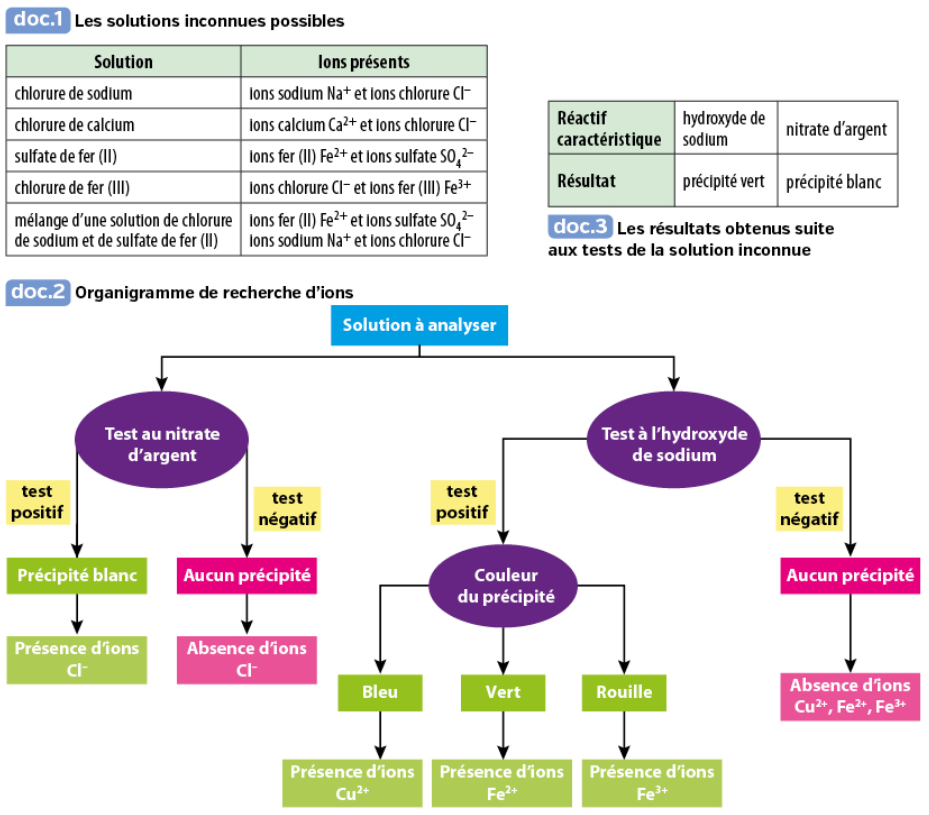
\includegraphics[scale=0.7]{img/docs}
		%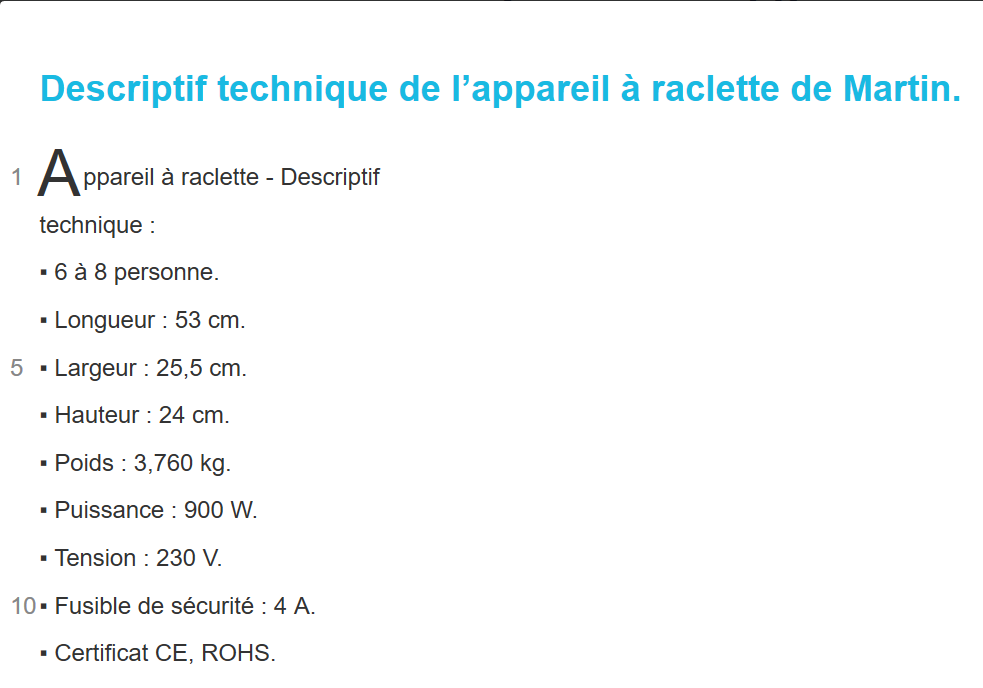
\includegraphics[scale=0.5]{img/doc2}
	\end{center}
%\end{multicols}

\begin{questions}
	\question[1] Quelles informations du descriptif technique permettront de savoir quelle sera la résistance appropriée ?
	
	\question[1\half] Quelle valeur de résistance correspond à l'intensité maximale ?
	
	\question[1\half] Quelle résistance devra choisir Martin ?
	
	\question[1] Que se passerait-il s'il choisissait l'autre ?
\end{questions}